\textit{Alvarenga p649 - Ejercicio 17}
\begin{enumerate}
    \item Una persona, de pie sobre el suelo, se encuentra a una distancia de $120 cm$ de un espejo plano vertical. Si se aleja el espejo de la persona una distancia igual a $40 cm$ (véase figura de este problema), ¿qué desplazamiento ocurrirá en la imagen de la persona?
    \item Para generalizar el resultado de la pregunta (a), suponga que la persona está a una distancia cualquiera del espejo plano. Si se aleja el espejo una distancia d, la imagen de la persona sufrirá un cambio $D$. Demuestre que $D = 2d$, cualquiera que fuese la distancia inicial de la persona respecto al espejo.
    \item La respuesta que encontró para la pregunta (a), ¿está de acuerdo con el resultado demostrado en (b)?
\end{enumerate}
\begin{figure}[h!]
\centering
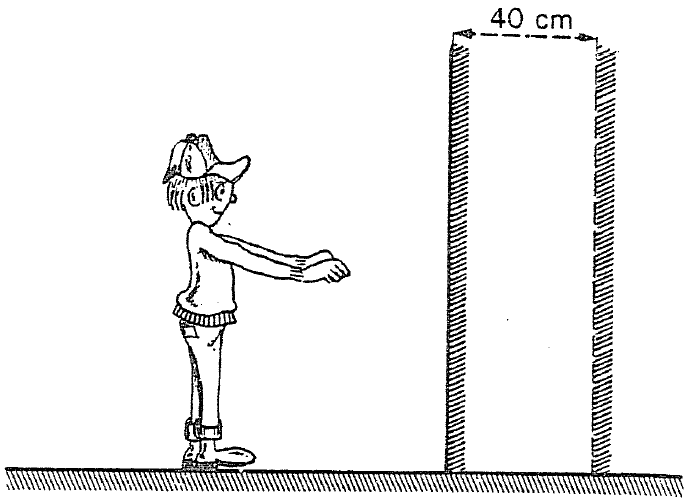
\includegraphics[width=0.4\linewidth]{Prob17_alvarenga649.png}
 \caption{Problema 10}
\end{figure}